% Figure audit of the GT2027 draft manuscript (the working draft in manuscript/), 27 Nov 2026.
% Build: pdflatex figure_audit.tex (twice). Diagrams are drawn inline with TikZ; no external figures.
\documentclass[10pt]{article}
\usepackage[utf8]{inputenc}
\usepackage[T1]{fontenc}
\usepackage{lmodern}
\usepackage{textcomp}
\usepackage[a4paper,margin=16mm]{geometry}
\usepackage{amsmath,amssymb}
\usepackage{booktabs,array,longtable,tabularx,enumitem,float}
\usepackage[dvipsnames]{xcolor}
\usepackage{tikz}
\usetikzlibrary{positioning,arrows.meta}
\usepackage[colorlinks=true,linkcolor=MidnightBlue,urlcolor=MidnightBlue]{hyperref}
\setlength{\parskip}{4pt}
\setlength{\parindent}{0pt}
\setlist{itemsep=1pt,topsep=2pt}
\setlength{\emergencystretch}{2em}
\renewcommand{\arraystretch}{1.12}
\setlength{\tabcolsep}{3pt}
\newcolumntype{L}[1]{>{\raggedright\arraybackslash}p{#1}}
\definecolor{oiBlue}{HTML}{0072B2}\definecolor{oiOrange}{HTML}{E69F00}\definecolor{oiGreen}{HTML}{009E73}
\definecolor{oiVerm}{HTML}{D55E00}\definecolor{oiSky}{HTML}{56B4E9}\definecolor{oiPink}{HTML}{CC79A7}

\title{GT2027 draft: figure audit against the claims}
\author{}
\date{27 November 2026}

\begin{document}
\maketitle
\vspace{-12mm}

\section*{Status}
Audit complete; decisions applied to \texttt{manuscript/main\_claude.tex} and mirrored in
\texttt{planning/writeup\_plan.tex}. Figure floats 17 $\rightarrow$ 9 now, 8 after the merge redraw; tables 2
$\rightarrow$ 2. Stand-in build 17 pages before (18 with the spots figure at full width) $\rightarrow$ 14 pages now,
an estimated 12.5--13 pages after the four pending redraws. Target 15 pages: met with about two pages of margin.

Inputs: \texttt{CLAUDE.md}, the writing style guide, the memory notes on framing, numbers, plan format and neutral
voice, \texttt{main\_claude.tex} and its PDF, \texttt{writeup\_plan.tex}, \texttt{story\_check.tex}, the archived plan
of 27 Nov, the CRVP literature note, the 40\_/41\_/42\_ previews in \texttt{planning/review/}, the data tables in
\texttt{figures/code/data/}, \texttt{planning/tracking.md} and the methods and validation drafts in
\texttt{4dns\_filmcooled/write\_up/}.

Rules, fixed before judging and applied in order: (i) a figure or panel that carries no claim of the abstract, aims or
conclusions is dropped, unless needed to understand the configuration or method; (ii) where three or more figures or
panels carry one claim, the one or two most direct are kept; (iii) a panel that repeats another figure is removed or
merged; (iv) a figure whose content fits one sentence or one table row becomes that sentence or row; (v) a
full-width figure must earn its width.

%=====================================================================================================
\section*{1\quad Claim list}
Source: A abstract, Ai aim, C conclusion item. K1--K14 are claims of the abstract, aims or conclusions; R1--R7 are
claims made only in results paragraphs.

{\footnotesize
\begin{longtable}{@{}L{0.7cm} L{12.6cm} L{3.4cm}@{}}
\toprule
\# & Claim & Source \\
\midrule
\endhead
K1 & Known RANS deficiencies are budgeted against one validated 193M reference. & A, Ai1--4 (framing) \\
K2 & From 20M points, the scale-resolving $\bar\eta$ agrees with the reference within 0.008 and with the experiment. & A, C1, Ai1 \\
K3 & The reference resolves the film ($\Delta/\eta_K\le2$); the 20M mesh does not over much of the film. & C1, Ai1 \\
K4 & The RANS is mesh-independent, 29--33\,\% low beyond $x/D=7$, with a centreline that is too high. & A, C1 \\
K5 & Through $z_x$, turbulence carries more coolant off the wall than the mean flow from $x/D=4.3$ in the reference, never in the RANS. & A, C2, Ai2 \\
K6 & The RANS velocity alone and its coolant distribution alone each raise the mean upwash flux by a similar factor. & A, C2 \\
K7 & A stronger inward mean sweep and, near the hole, a weaker outward turbulent flux narrow the plume (0.75 width at $x/D=20$). & A, C2, Ai2 \\
K8 & The budgets are consistent with a CRVP of 1.2--1.8 times the reference circulation. & C2 (Intro gap) \\
K9 & Near the wall the RANS eddy viscosity is 0.55--0.66 of the reference, mostly a short length; the assumed alignment offsets part. & A, C3, Ai3 \\
K10 & Above $z_x$ the factor errors cancel in the eddy viscosity. & C3, Ai3 \\
K11 & The reference classic $\Pr_t$ is 0.23--0.45 in the film against the setting of 0.9. & A, C3, Ai3 \\
K12 & A lower $\Pr_t$ corrects the centreline but not the spread. & A, C4, Ai4 \\
K13 & QCR with $\Pr_t=0.4$ matches $\bar\eta$ with a film that is too narrow; $\bar\eta$ alone is not sufficient evidence. & C4, Ai4 \\
K14 & A resolved heat flux imposed in the film recovers the film shape. & A, C4, Ai4 \\
\midrule
R1 & Three named mean features (CRVP, HV, WV); the RANS isosurface is smooth. & 4 lead-in \\
R2 & The RANS diffuser separates less and passes 4.7\,\% more coolant; small against the deficit. & 4.1 hole \\
R3 & The windward shear layer rolls up and breaks down by $x/D\sim3$. & 4.1 jet \\
R4 & The RANS mid-pitch layer stays laminar; the reference and the LES transition alike between the jets. & 4.1 layer \\
R5 & The short RANS length is a short dissipation length; location across the span. & 4.2 \\
R6 & Heat diffusivity anisotropic on the flanks; RANS lateral diffusivity deficit mostly the $\Pr_t$ setting. & 4.2 spanwise \\
R7 & $\Pr_t$ below 0.3 along the jet core, at or above 0.9 only in a thin wall layer. & 4.2 $\Pr_t$ \\
\bottomrule
\end{longtable}}

%=====================================================================================================
\section*{2\quad Claim-to-figure matrix}
P: primary carrier; S: second carrier; Rp: repeats another figure; --: none. Use: \textbf{U} cited with something
to look at; \textbf{M} mentioned only.

{\footnotesize
\begin{longtable}{@{}L{1.0cm} L{3.9cm} L{0.9cm} L{3.4cm} L{0.7cm} L{6.3cm}@{}}
\toprule
Fig. & Content (panel) & Width & Claims carried & Use & Note \\
\midrule
\endhead
F1 & configuration, regions & full & method & U & needed for the configuration \\
T1 & simulations, meshes & full & K4 (mesh-indep.), R2 (BR) & U & method \\
F2a & resolution, diffuser & full & -- (diffuser fact) & U & fact fits a sentence (already in text) \\
F2b & resolution, exit & full & -- & -- & not cited \\
F2c,d & resolution, near/far film & full & K3 P & U & far film labelled 10--25 in the file \\
F2e & resolution, whole domain & full & -- & -- & not cited \\
F3 & 3D mean flow, RANS and 193M & col., 6.1\,in & R1 (K8 visual, Rp of F7 top b) & U & names CRVP, HV, WV; HV unused later \\
F4 & hole axis $C_p$, reversed area & col. & R2 & U & numbers fit one sentence; BR in T1 \\
F5a & $\bar\eta$ & col. & K2 P, K4 P & U & \\
F5b & centreline $\eta$ & col. & K4 P & U & \\
F5c & mid-pitch $\eta$, $\gamma$ & col. & K4 S, R4 S & U & carries the reference $\gamma$ \\
F6 & instantaneous centre plane & col. & R3 & M & no claim beyond R3 \\
F7 top a & core positions & full & K8 (0.1$D$ lower) & U & one number \\
F7 top b & circulation CRVP, WV & full & K8 P & U & the circulation ratio is a stated contribution \\
F7 bot a & vertical flux through $z_x$ & full & K5 P & U & \\
F7 bot b & RANS/193M ratios & full & K7 (width 0.75), K4 Rp & U & $\bar\eta$ and centreline ratios repeat F5 \\
F8a & swap test & col. & K6 P & U & \\
F8b & lateral budget & col. & K7 P & U & \\
F9 & $H$, $C_f$, centreline and mid-pitch & full & R4 & U & not in abstract or conclusions \\
F10 & spots: snapshots, $x$--$t$, $\gamma$ & full, 7.75\,in & R4 (Rp of F5c for $\gamma$) & U & most of a page \\
F11a--c & ratio maps $k^{1/2}$, $L$, $1/\cos\theta$ & full & K10 P & U & above $z_x$: three numbers \\
F11d & ratio map $\mu$, $z_x$ & full & K9 S, method ($z_x$) & U & defines the near-wall layer \\
F12a & log split below $z_x$ & col. & K9 P & U & \\
F12b & factor ratios below $z_x$ & col. & K9 P & U & \\
F13 & cross-planes $k$, $L_{\mathrm{eff}}$ & col. & R5, K9 Rp & U & third carrier of the short length \\
F14 & $\Pr_t$ span map & col. & K11 S, R7 & U & spatial picture, not a row \\
F15 & regional $\Pr_{t,R}$ & col. & K11 P & U & six numbers and reference lines: one table row \\
F16a & diffusivity ratios & full & R6 & U & not in abstract or conclusions \\
F16b & lateral heat-flux split & full & R6 & U & medium confidence \\
T2 & a posteriori runs & full & K12, K13, K14 P & U & \\
F17a & $\bar\eta$ & full & K13 S & U & \\
F17b & centreline $\eta$ & full & K12 Rp (T2, F17d at $y=0$) & U & \\
F17c & mid-pitch $\eta$ & full & K12, K14 S & U & \\
F17d & lateral profile & full & K12, K13, K14 P & U & \\
\bottomrule
\end{longtable}}

%=====================================================================================================
\section*{3\quad Decisions}
{\footnotesize
\begin{longtable}{@{}L{1.0cm} L{3.0cm} L{1.4cm} L{11.2cm}@{}}
\toprule
Fig. & Decision & Claims & Reason \\
\midrule
\endhead
F1 & KEEP & method & Needed for the configuration; redrawn without boundary-condition notes (final file in). \\
T1 & KEEP & K4, R2 & Method; carries the BR of every simulation. \\
F2 & KEEP FEWER PANELS: (c), (d) & K3 & Rule (v): two of five panels carry K3; (b), (e) uncited; (a) diffuser fact is a sentence (iv). Column width. \\
F3 & DROP & R1 & Rule (i): no abstract or conclusion claim; WV defined in the text; CRVP strength carried by F7 top b (iii). \\
F4 & DROP & R2 & Rules (i), (iv): one sentence plus Table 1. \\
F5 & KEEP & K2, K4 & Primary carrier of validation and of the RANS deficit; (c) also carries the reference $\gamma$. \\
F6 & DROP & R3 & Rule (i); one clause kept. \\
F7 & MERGE with F8, fewer panels & K5, K8 & Rule (iii): top a is one number, bottom b repeats F5 except the 0.75 width (iv). Keep top b and bottom a. \\
F8 & MERGE into F7 & K6, K7 & One four-panel full-width row replaces a 0.7-width two-row float and a column float (v). \\
F9 & DROP & R4 & Rule (i); findings kept as two sentences. \\
F10 & DROP & R4 & Rules (i), (iii): its $\gamma$ panel repeats F5c; full width, most of a page. \\
F11 & KEEP FEWER PANELS: (d) & K9, K10 & Rule (iv): above-$z_x$ factor ratios are three numbers (now in the text and, after the redraw, in F12b); (d) defines $z_x$. Column width. \\
F12 & KEEP, add above-$z_x$ lines (MERGE) & K9, K10 & Primary for K9; absorbs the K10 content of F11a--c. \\
F13 & DROP & R5 & Rule (ii): third carrier of the short length after F12 and F11; finding kept as a sentence. \\
F14 & KEEP & K11, R7 & One $\Pr_t$ figure; the spatial pattern does not fit a row. \\
F15 & DROP & K11 & Rule (iv): six numbers, now one sentence (volume and centre-plane values). \\
F16 & DROP & R6 & Rule (i); two sentences kept, with the medium confidence. \\
T2 & KEEP & K12--14 & Primary carrier of 4.3. \\
F17 & KEEP FEWER PANELS: (a), (c), (d) & K12--14 & Rule (iii): (b) repeats T2 and F17d at $y=0$; one row of three at full width. \\
\bottomrule
\end{longtable}}

\begin{figure}[H]
\centering
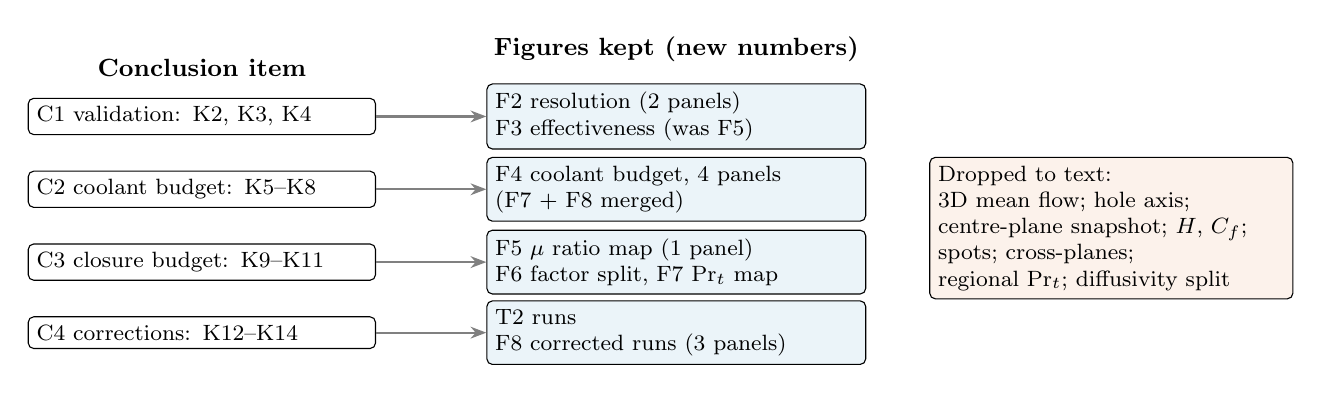
\begin{tikzpicture}[
  every node/.style={font=\footnotesize},
  cl/.style={draw, rounded corners=2pt, text width=4.2cm, align=left, inner sep=3pt},
  fg/.style={draw, rounded corners=2pt, text width=4.6cm, align=left, inner sep=3pt, fill=oiBlue!8},
  dr/.style={draw, rounded corners=2pt, text width=4.4cm, align=left, inner sep=3pt, fill=oiVerm!8},
  arr/.style={-{Stealth[length=2mm]}, gray, thick}]
\node[cl] (c1) {C1 validation: K2, K3, K4};
\node[cl, below=0.45cm of c1] (c2) {C2 coolant budget: K5--K8};
\node[cl, below=0.45cm of c2] (c3) {C3 closure budget: K9--K11};
\node[cl, below=0.45cm of c3] (c4) {C4 corrections: K12--K14};
\node[fg, right=1.4cm of c1] (f1) {F2 resolution (2 panels)\\ F3 effectiveness (was F5)};
\node[fg, right=1.4cm of c2] (f2) {F4 coolant budget, 4 panels\\ (F7 + F8 merged)};
\node[fg, right=1.4cm of c3] (f3) {F5 $\mu$ ratio map (1 panel)\\ F6 factor split, F7 $\Pr_t$ map};
\node[fg, right=1.4cm of c4] (f4) {T2 runs\\ F8 corrected runs (3 panels)};
\foreach \a/\b in {c1/f1,c2/f2,c3/f3,c4/f4} \draw[arr] (\a) -- (\b);
\node[dr, right=0.8cm of f2.north east, anchor=north west] (d) {Dropped to text:\\ 3D mean flow; hole axis;\\
centre-plane snapshot; $H$, $C_f$;\\ spots; cross-planes;\\ regional $\Pr_t$; diffusivity split};
\node[font=\small\bfseries, above=0.15cm of c1] {Conclusion item};
\node[font=\small\bfseries, above=0.15cm of f1] {Figures kept (new numbers)};
\end{tikzpicture}
\caption{Each conclusion item and the figures that carry it after the audit; one or two figures per item. Right:
figures whose findings are now sentences.}
\end{figure}

%=====================================================================================================
\section*{4\quad Omissions}
Classes: TEXT restore as text (done); ROW restore as a table row; FIG/COMP needs a figure or a computation (listed
for the owner); OUT leave out.

{\footnotesize
\begin{longtable}{@{}L{4.4cm} L{1.2cm} L{11.0cm}@{}}
\toprule
Omission & Class & Action \\
\midrule
\endhead
Time integration, initialisation, flush, averaging & TEXT + open & Added to 3.1: Courant number 1.0; 50M 3DNS from the RANS, 100M and 193M from the 50M (mass flux within 0.006\,\%), 20M LES from the 100M; flush 3.35\,FT (50M), $\ge$1\,FT (finer); averaging per Table 1. Scheme name not in the files: \texttt{\%\% OPEN}. \\
Mesh and resolution numbers for aim 1 & TEXT + COMP & Added: hole cross-section 0.4--2.5 wall units (100M, 193M). Volume fractions per mesh and region, plate wall units per mesh and the 5M curve: computation for the owner (existing open marker kept). \\
Experiment conditions and uncertainty & TEXT + open & Added in 4.1: Tu 0.5\,\%, Mach 0.03, $Re_D\approx4960$, tripped layer $Re_\theta$ 630--700, $\pm0.024$ in $\eta$ (95\,\%), up to $\pm6.5$\,\% in BR; 0.008 agreement stated as a third of the uncertainty. Source of the uncertainty (2014 or 2015 paper) to confirm: \texttt{\%\% OPEN}. \\
193M uncertainty & TEXT & Added in 3.1: delete-one jackknife over ten 1-FT batches; record-length check (0.046) already in 4. \\
Optimal eddy viscosity and mask & present & Eq.~8 definition, literature, strain mask, manual jet-edge mask and passed fraction already stated. No action. \\
$y$-uniform span averaging & present & Stated in 3.1. No action. \\
Flux ratios against surface height & TEXT & Added: at $z/D=1.0$ RANS turbulent flux 0.67--0.98 of the reference; at $z/D=0.25$ towards the wall. \\
Control-volume balance residual & TEXT & Added: reference coolant balance below $z/D=0.5$ closes within 5\,\% at every station, median 1.2\,\% (N7, \texttt{tracking.md}). \\
Operating-point limits of the guidance & TEXT & Added at the head of 4.3.4: flat plate, ZPG, BR 1.5, DR 1.5, VR $\sim$1, laminar approach, Tu 5.5\,\%, SST with $\gamma$--$Re_\theta$; untested transfer named. \\
Boundary conditions (from the configuration figure) & TEXT & Added: domain $x/D$ $-15$ to 25, $z/D$ 10, span $6D$; Blasius inlet $Re_\theta$ 135--140; outlet and top at free-stream static pressure, characteristic in 3DNS; adiabatic no-slip walls; coolant turbulence 12.5--15\,\% (3DNS), 15\,\% (STAR-CCM+); metering/diffuser split $3.5D$ from the breakout. \\
Archived plan: CRVP velocities & TEXT & Added: RANS centreline upwash at core height 1.14--1.66 times, inward velocity at $z/D=0.1$ 1.75--1.93 times (\texttt{mean\_features\_table.txt}). \\
Archived plan: above-$z_x$ factors & TEXT & Added: film mean $\mu$ 1.07, $k^{1/2}$ 1.13, length 0.81, $1/\cos\theta$ 1.30 (\texttt{meff\_maps\_table.txt}). \\
Archived plan: centre-plane $\Pr_t$ & TEXT & Added: 0.44, 0.63, 0.80 with the volume values. \\
Archived plan: BR-matched RANS & COMP & Prepared 9 Nov, no result in the files; would separate the 4.7\,\% BR effect from the model. For the owner. \\
Archived plan: literature value of best-practice RANS $\bar\eta$ error & COMP (search) & Open marker in the Introduction kept. \\
Literature counter-evidence & TEXT & Added: weaker $k$--$\varepsilon$ pair without more spreading (Stratton and Shih 2019); Reynolds-stress models did not widen the film (Acharya 2001; Harrison and Bogard 2008). Foroutan and Milani already in the Introduction. \\
Discharge coefficient, slow mode, spot celerities & OUT & Support no abstract or conclusion claim. \\
Three a posteriori runs ($\Pr_t$ 0.4 in film, stresses alone, $\gamma=1$) & COMP & Running; stated as incomplete in 4.3. \\
\bottomrule
\end{longtable}}

%=====================================================================================================
\section*{5\quad Figure requests (for the figure agent)}
Each request is also a \texttt{\%\% FIGURE REQUEST} comment above its float in \texttt{main\_claude.tex}; captions and
panel letters in the text change only after the redraw.
\begin{enumerate}[label=\arabic*.]
\item \texttt{fig\_resolution.pdf}: keep (c) near film and (d) far film only; far film recomputed over $x/D$
  10.25--20 (the file labels 10--25); near film labelled 2.36--10.25; add the 5M if its mapping exists; two panels
  side by side, shared $y$ axis, for \texttt{\textbackslash columnwidth}, $\sim$2.3\,in tall. Float becomes one column.
\item New \texttt{fig\_coolant\_budget.pdf} (merge of \texttt{fig\_mean\_features}, \texttt{fig\_flux\_eta},
  \texttt{fig\_swap\_lateral}): one row of four panels for \texttt{\textbackslash textwidth}, $\sim$2.4\,in tall,
  shared legend below: (a) $\Gamma$ of the CRVP and WV; (b) vertical flux through $z_x$, mean and turbulent, with
  band; (c) swap test; (d) lateral flux below $z_x$ at $|y|=0.5D$, with band. Removed: core positions and the
  ratio panel. The \texttt{fig:swap} float is then deleted.
\item \texttt{fig\_meff\_maps.png}: keep (d) the eddy-viscosity ratio with $z_x$ and the grey mask; for
  \texttt{\textbackslash columnwidth}, $\sim$1.6\,in tall, colour bar right. Float becomes one column.
\item \texttt{fig\_meff\_split\_film.pdf}: add to (b), as dashed lines, the factor ratios of the layer above $z_x$
  in slabs of $1D$ (data in \texttt{meff\_maps\_table.txt}); below $z_x$ solid; both labelled.
\item \texttt{fig\_aposteriori.pdf}: keep (a) $\bar\eta$, (c) mid-pitch, (d) lateral profile; one row of three for
  \texttt{\textbackslash textwidth}, $\sim$2.4\,in tall, legend below.
\end{enumerate}

%=====================================================================================================
\section*{6\quad Counts}
\begin{figure}[H]
\centering
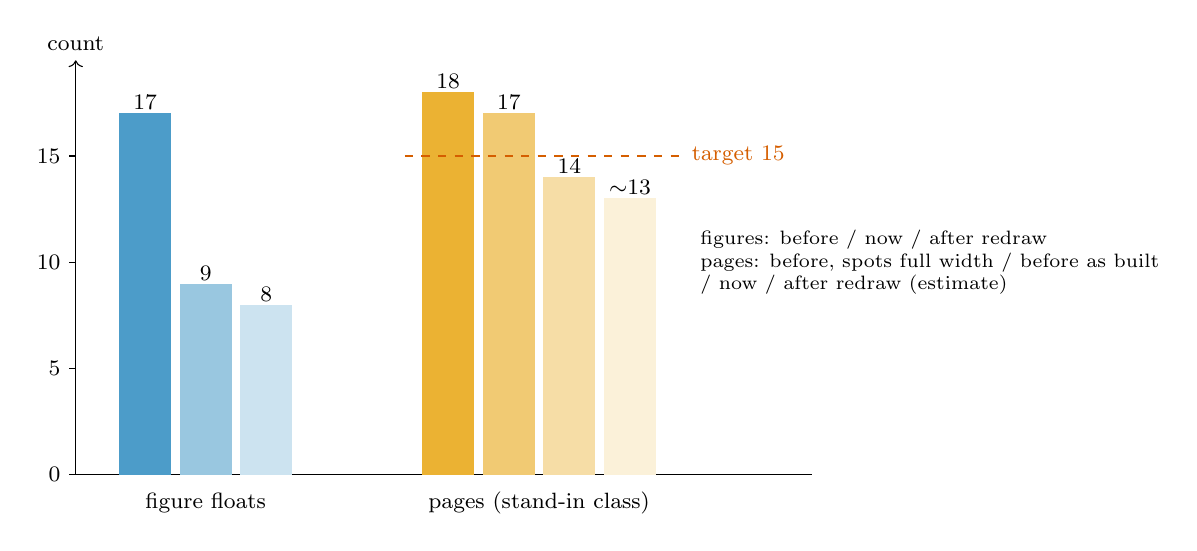
\begin{tikzpicture}[x=0.55cm,y=0.27cm, every node/.style={font=\footnotesize}]
\draw[->] (0,0) -- (0,19.5) node[above] {count};
\foreach \y in {0,5,10,15} \draw (-0.15,\y) -- (0,\y) node[left=2pt] {\y};
\draw (0,0) -- (17,0);
% figures
\fill[oiBlue!70] (1,0) rectangle (2.2,17); \node at (1.6,17.5) {17};
\fill[oiBlue!40] (2.4,0) rectangle (3.6,9); \node at (3.0,9.5) {9};
\fill[oiBlue!20] (3.8,0) rectangle (5.0,8); \node at (4.4,8.5) {8};
\node[align=center] at (3.0,-1.3) {figure floats};
% pages
\fill[oiOrange!80] (8,0) rectangle (9.2,18); \node at (8.6,18.5) {18};
\fill[oiOrange!55] (9.4,0) rectangle (10.6,17); \node at (10,17.5) {17};
\fill[oiOrange!35] (10.8,0) rectangle (12.0,14); \node at (11.4,14.5) {14};
\fill[oiOrange!15] (12.2,0) rectangle (13.4,13); \node at (12.8,13.5) {$\sim$13};
\node[align=center] at (10.7,-1.3) {pages (stand-in class)};
\draw[dashed, oiVerm] (7.6,15) -- (14,15) node[right] {target 15};
\node[align=left, anchor=west, font=\scriptsize] at (14.2,10) {figures: before / now / after redraw\\
pages: before, spots full width / before as built\\ / now / after redraw (estimate)};
\end{tikzpicture}
\caption{Figure floats and pages before the audit, now, and after the five redraws. Before: 17 figure floats
(18 image files) and 2 tables.}
\end{figure}

Estimate of the redraw savings, in page fractions of a 9\,in text height: merged coolant budget $-0.55$; eddy-viscosity
map to one column $-0.4$; a posteriori to one row $-0.35$; resolution to one column $-0.15$; total about $-1.45$.
The margin of about two pages allows the owner to reinstate one dropped figure: the 3D mean flow (F3, $\sim$0.33
page) is the candidate if a picture of the flow is wanted.

\end{document}
